
\documentclass{article}
\usepackage[spanish]{babel} %Definir idioma español
\usepackage[utf8]{inputenc} %Codificacion utf-8
\usepackage{amssymb, amsmath, amsbsy, wasysym}
\usepackage{multirow} % para tablas
\usepackage{graphicx}
\title{Práctica 1//Redes de computadoras}
\author{Emmanuel Peto Gutiérrez}
\begin{document}
\maketitle

\section{Pasos para realizar la práctica}

Se instalaron los software: Virtual Box, Vagrant y Wireshark.

Se clonó el repositorio \texttt{https://gitlab.com/ismael.andrade/redes-2021-1.git} y en la sección \texttt{lab1}, en mi computadora, se ejecutó el comando \texttt{vagrant up}; sin embargo, se obtuvo el siguiente error que no se supo corregir: \textit{A host only network interface you're attempting to configure via DHCP already has a conflicting host only adapter with DHCP enabled. The DHCP on this adapter is incompatible with the DHCP settings. Two host only network interfaces are not allowed to overlap, and each host only network interface can have only one DHCP server. Please reconfigure your host only network or remove the virtual machine using the other host only network.}

\begin{center}
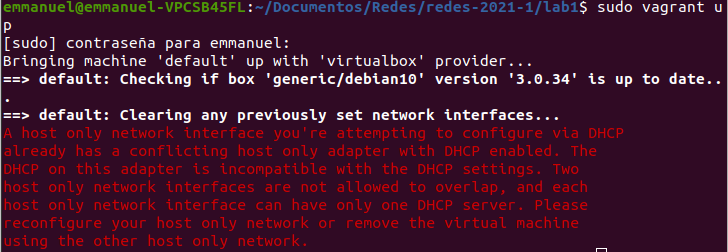
\includegraphics[width=\linewidth]{imagenes/error_vagrantup}
\end{center}

Dado el error, se procedió a instalar manualmente la máquina virtual de Debian 10 en Virtual Box, descargando el ISO de la página de Debian.

\begin{center}
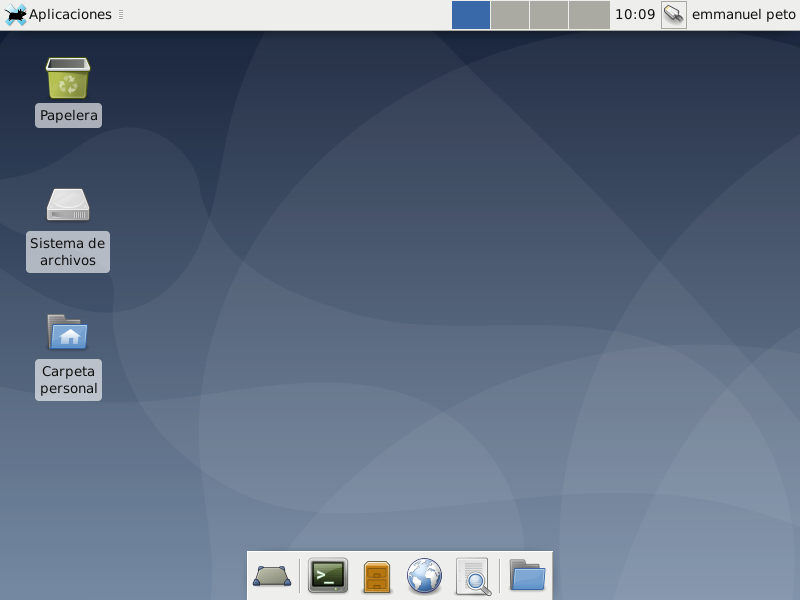
\includegraphics[width=\linewidth]{imagenes/VirtualBox_Debian}
\end{center}

Para conocer las direcciones, MAC e IP, se ejecutó el comando \texttt{ip addr}.

En la computadora:

\begin{center}
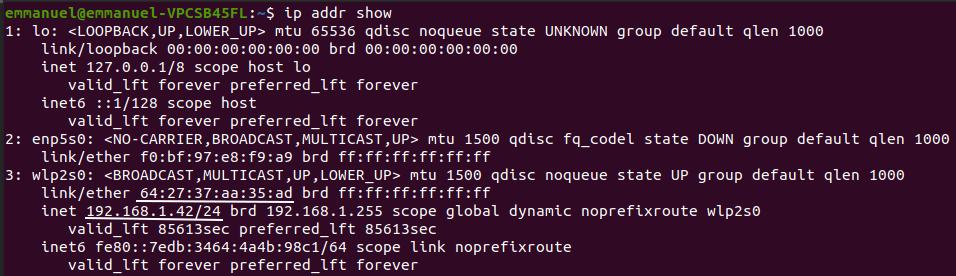
\includegraphics[width=\linewidth]{imagenes/direcciones_local}
\end{center}

En la máquina virtual:

\begin{center}
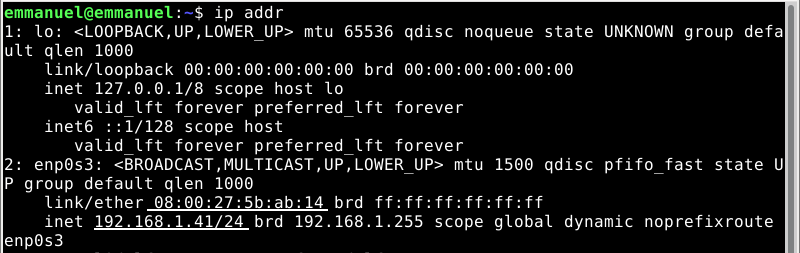
\includegraphics[width=\linewidth]{imagenes/direcciones_virtual2}
\end{center}

Se abrió Wireshark para capturar el tráfico. Se intentó entrar a vboxnet0 y vboxnet1.

\begin{center}
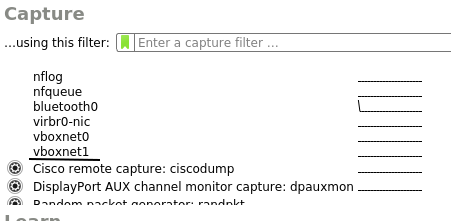
\includegraphics[width=\linewidth]{imagenes/ws_vbnet}
\end{center}

Sin embargo, se obtuvieron los siguientes errores:

\begin{center}
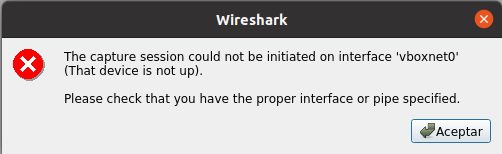
\includegraphics[width=0.45\linewidth]{imagenes/errorvbnet1}
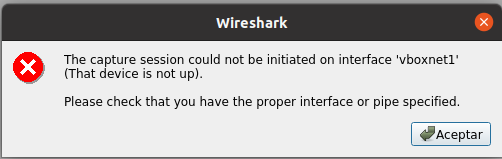
\includegraphics[width=0.45\linewidth]{imagenes/errorvbnet2}
\end{center}

Así que se optó por \texttt{wlp2s0}. En esta opción, se aplicó el filtro ARP.

\begin{center}
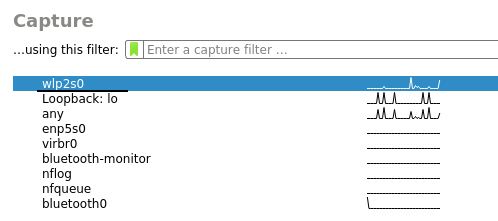
\includegraphics[width=\linewidth]{imagenes/ws_wlp}
\end{center}

Posteriormente se procedió a hacer ping desde mi máquina (192.168.1.42) hacia la máquina virtual (192.168.1.41).

\begin{center}
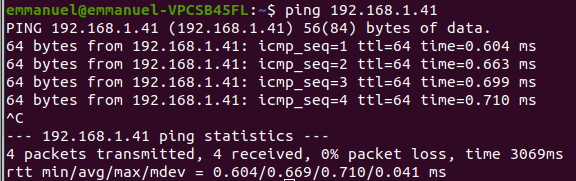
\includegraphics[width=\linewidth]{imagenes/ping}
\end{center}

Se puede observar el tráfico generado por el ping, en Wireshark.

\begin{center}
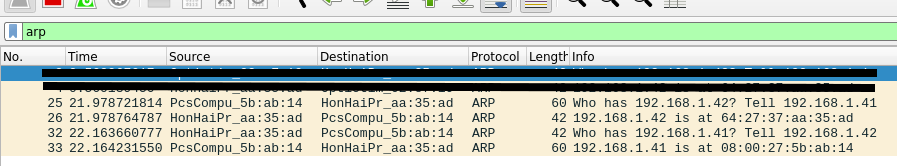
\includegraphics[width=\linewidth]{imagenes/captura_wireshark2}
\end{center}

\section{Cuestionario}

\textbf{1. ¿Cuáles son las direcciones físicas de tu equipo y de la máquina virtual?}

\begin{itemize}
\item La de mi equipo es \texttt{64:27:37:aa:35:ad}.
\item La de la máquina virtual es \texttt{08:00:27:5b:ab:14}.
\end{itemize}

\textbf{2. ¿Cúales son las direcciones lógicas de tu equipo y la máquina virtual?}

\begin{itemize}
\item La de mi equipo es \texttt{192.168.1.42}.
\item La de la máquina virtual es \texttt{192.168.1.41}.
\end{itemize}

\textbf{3. ¿Cuál es la diferencia a nivel de bits entre una dirección física y una lógica?}

A nivel de bits se diferencian por la cantidad que una usa respecto a la otra. En la dirección MAC se usan 6 bloques de 8 bits, o sea 48 bits. La dirección IPv4 usa 4 bloques de 8 bits, o sea 32 bits.\\

\textbf{4. ¿Por qué existen dos consultas ARP?}

Porque primero, el dispositivo que realizó el ping (192.168.1.42) pregunta cuál es la dirección MAC del dispositivo al que envió el ping (192.168.1.41). Después, el dispositivo que recibe el ping envía un mensaje de regreso y debe preguntar por la dirección MAC de 192.168.1.42. Así, en este caso, se deben traducir las direcciónes de la computadora y de la máquina virtual.\\

\textbf{5. Investigar y describir de manera breve en que consiste un ataque de ARP spoofing.}

Un atacante en una red se coloca como intermediario entre las comunicaciones de un dispositivo y un router.\\

\textbf{6. Investigar el fabricante del adaptador de red físico del equipo personal.}

El del wireless: Qualcomm Atheros.

El del Ethernet: Realtek Semiconductor Co., Ltd.

\end{document}

